LazySets provides ways to convert one set representation to another.
If a conversion is not possible due to restrictions in the represented class of sets, LazySets provides ways to obtain approximations.
Turning to an approximate but simpler set representation is also interesting for answering questions efficiently that would otherwise be computationally expensive.


\subsection{Conversion}

LazySets extends Julia's \code{convert} function for converting between set representations. The first argument is the target type and the second argument is the source set.
%
Below are three mathematically equivalent representations of the interval $\X = [0, 1] \subseteq \R$:

\begin{minipage}{\linewidth}
	\vspace{-\abovedisplayskip}
	\begin{lstlisting}
julia> X = Interval(0, 1)
Interval{Float64,
  IntervalArithmetic.Interval{Float64}}([0, 1])

julia> convert(Hyperrectangle, X)
Hyperrectangle{Float64, Vector{Float64},
  Vector{Float64}}([0.5], [0.5])

julia> convert(Zonotope, X)
Zonotope{Float64, Vector{Float64},
  Matrix{Float64}}([0.5], [0.5])
	\end{lstlisting}
\end{minipage}
There are even more possibilities, such as representing $\X$ as an intersection of half-spaces (try \code{convert(HPolytope, X)}).


\smallskip

With multiple dispatch it is easy to define less obvious conversions, e.g., to convert the Cartesian product of an interval and a two-dimensional hyperrectangle to a three-dimensional zonotope:

\begin{minipage}{\linewidth}
	\vspace{-\abovedisplayskip}
	\begin{lstlisting}
julia> X = rand(Interval)

julia> Y = rand(Hyperrectangle, dim=2)

julia> Z = convert(Zonotope, X × Y)
Zonotope{Float64, ...}

julia> dim(Z)
3
\end{lstlisting}
\end{minipage}


\subsection{Approximation}\label{sec:approximation}

\begin{figure}
	\hfill
	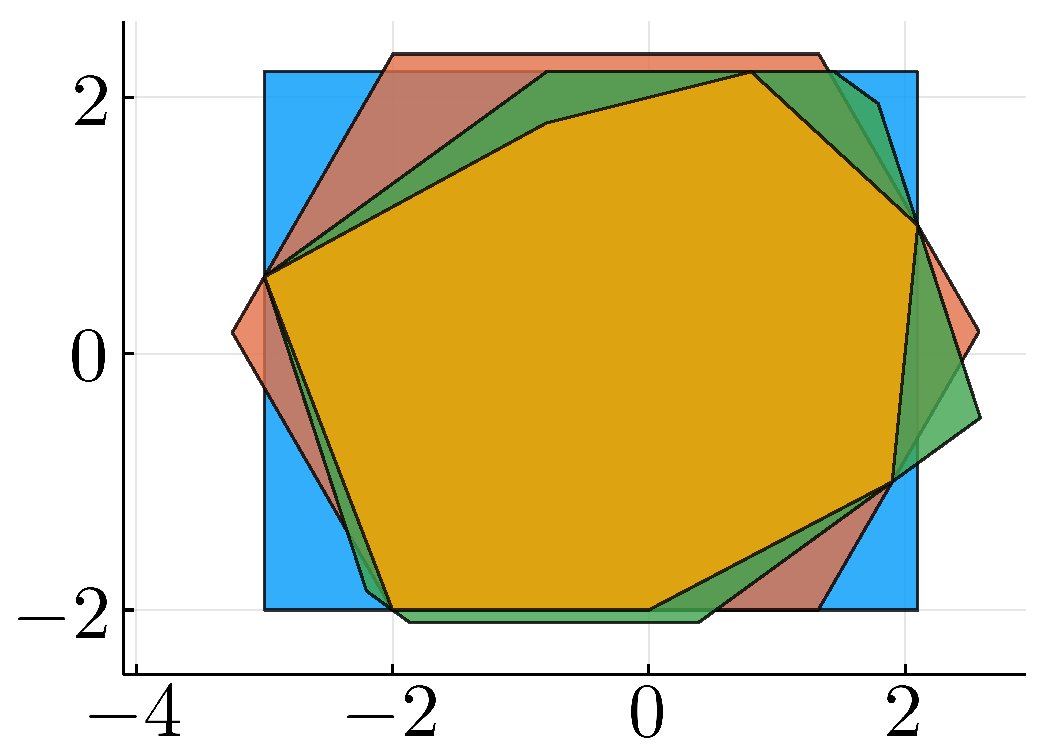
\includegraphics[height=30mm]{img/overapproximate}
	\hfill
	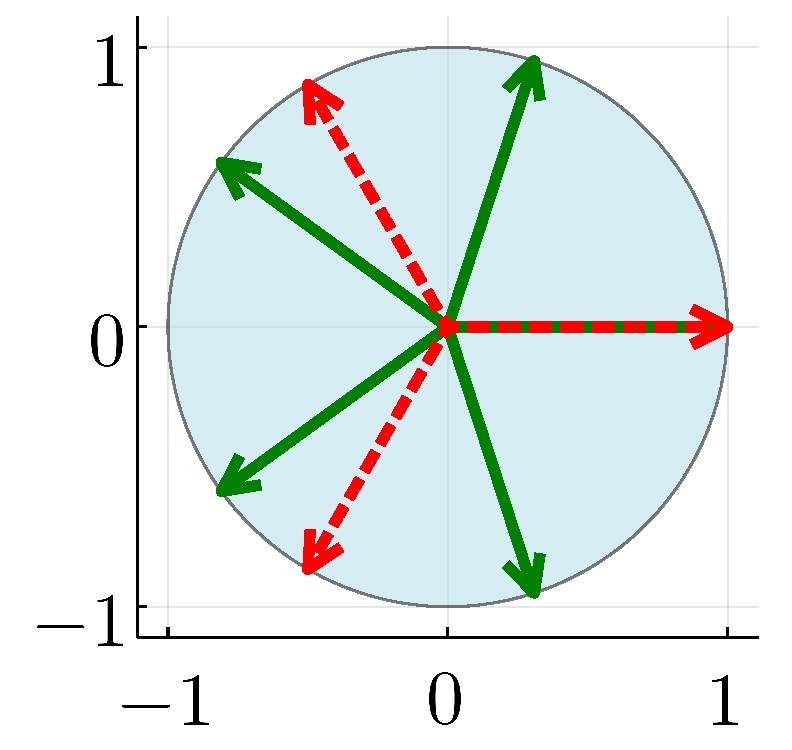
\includegraphics[height=30mm]{img/polardirs}
	\hfill\
	\vspace*{1mm}
	\caption{Left picture: Overapproximation of the polytope from Fig.~\ref{fig:supfunc} (orange) with a hyperrectangle (blue) and two zonotopes. The zonotope generators were synthesized from three (red) resp.\ five (green) polar directions (right). Observe that the approximations are pairwise incomparable.}
	\label{fig:overapproximate}
\end{figure}

In many applications we do not require exact results but are content with an approximation. To still give mathematical guarantees, one usually aims for either over- or underapproximations.

We can use the support function to get an overapproximation: For every nonempty compact convex set $X \subseteq \R^n$ and $D \subseteq \R^n$ we have
\begin{equation*}
	X \subseteq \bigcap_{d \in D} \{d^T x \leq \rho(d, X)\}
\end{equation*}
and equality holds for $D = \R^n$.

\smallskip

LazySets has predefined common template directions such as \code{OctDirections(2)} for directions normal to a regular octagon in two dimensions. Fig.~\ref{fig:supfunc} (right) illustrates the evaluation of overapproximating the set $X$ with octagonal directions, resulting in a polygon with eight constraints. Apart from common fixed template directions there are also options for parametric uniform directions in two (\code{PolarDirections}) or three (\code{SphericalDirections}) dimensions or for a custom set of directions (\code{CustomDirections}).

\begin{minipage}{\linewidth}
\vspace{-\abovedisplayskip}
\begin{lstlisting}
julia> Xoct = overapproximate(X, OctDirections(2))

julia> length(constraints_list(Xoct))
8
\end{lstlisting}
\end{minipage}

In two dimensions, LazySets can compute $\varepsilon$-close overapproximations using a method by Kamenev~\cite{kamenev1996algorithm} later refined in~\cite{lotov2008modified}.
%
It is used via \code{overapproximate(X, $\varepsilon$)}, where $\varepsilon$ is the specified tolerance.
%
The higher-dimensional extension is not implemented yet.
%
On the other hand, higher-dimensional set can be lazily projected using the support function to a lower-dimensional subspace, where the available method applies.

\smallskip

In some applications, we may want to ensure that the result has a specific set type.
The smallest bounding box is available by specifying the second argument type. It yields a \code{Hyperrectangle}, which is more efficient to work with.

\begin{minipage}{\linewidth}
	\vspace{-\abovedisplayskip}
	\begin{lstlisting}
julia> overapproximate(X, Hyperrectangle)

julia> box_approximation(X) # alias
\end{lstlisting}
\end{minipage}

We can use \code{overapproximate(P, Zonotope, D)}, where \code{P} is a polytope and \code{D} is a vector of directions used as candidates for the generators, to obtain a zonotope (in any dimension). We show some example overapproximations in Fig.~\ref{fig:overapproximate}.
Underapproximations can be obtained using the function \code{underapproximate}.
